\documentclass[12pt,a4paper]{article} 
\usepackage{tikz}
\usepackage{float}
\usepackage{graphicx}
\usepackage{multirow}
\usepackage{setspace} 
\usepackage{graphicx}
\usepackage{times}
\pagenumbering{roman}
\usepackage{geometry}

\geometry{verbose,tmargin=2cm,bmargin=2cm,lmargin=3cm,rmargin=2cm}
\usepackage{fancyhdr} 
%\linespread{1.05} 
\usepackage{tikz}
\usetikzlibrary{arrows}
\usetikzlibrary{shapes.geometric}

\tikzstyle{kres} = [rectangle, rounded corners, minimum width=1cm, minimum height=0.5cm,text centered, draw=black]
\tikzstyle{nad} = [trapezium, trapezium left angle=60, trapezium right angle=100, minimum width=1cm, minimum height=0.5cm, text centered, draw=black]
\tikzstyle{sim} = [trapezium, trapezium left angle=60, trapezium right angle=100, minimum width=1cm, minimum height=0.5cm, text centered, draw=black]
\tikzstyle{garis} = [thick,->,>=stealth]
\usetikzlibrary{shapes,arrows}

\begin{document} % Mulai Penulisan Laporan
\onehalfspacing
\begin{titlepage}

\title{\textbf{LAPORAN PRAKTIKUM ELEKTRONIKA DASAR
\\ HUKUM OHM }}  %Judul Laporan
%\title{\textbf{FOTOKATALISIS}}  %Judul Laporan
\author{\textbf {Dosen : Mada Sanjaya WS, Ph.D }
\\ \textbf{Asisten Lab : Sri Rohmawati (1177030037)}
\\ \textbf{ }
\\ \textbf{Disusun Oleh :}
\\ \textbf{Muhamad Fahmi Adzkar} \textbf {(1187030024)}
\\ \textbf{Kelompok 6 :}
\\ \textbf{Hani Hikmawati} \textbf {(1187030014)}
\\ \textbf{Sri Rahayu} \textbf {(1187030036)}
\\ \textbf{Yuni Rahayu} \textbf {(1187030041)}}

\maketitle
\begin{center}
\vspace{1cm}

\includegraphics[width=4cm]{uin.png}
\vspace{1cm}

JURUSAN FISIKA\\
FAKULTAS SAINS DAN TEKNOLOGI\\
UIN SUNAN GUNUNG DJATI BANDUNG\\
2019\\
\end{center}
\end{titlepage}

\renewcommand\abstractname{Abstract} %Untuk Abstrak Bahasa Inggris
\begin{abstract}
Ohms law is a statement that a large current owing through a conductor is always directly propotional to the potential diference is applied. To calculate an obstacle, then the current and voltage of each circut are arranged in series and parallel advance as described in ex-perimental procedures. As for tools used in this lab are : protoboard,some resistors, multimeters, power supply and computers. It can be concluded that there is a continuous relationshipbetween an enlarged voltage electric current into the circuit by owing, both of wich are associated with a value that makes both of them have a xed ratio. this value was then called obstacles that ultimately led to a mathematical idea ohms law.

\subparagraph{ }
\textit{Keywords: Ohms law, series and parallel circuit, obstacle,voltage,electric current.}

\end{abstract}

\renewcommand\abstractname{Abstrak} %Untuk Abstrak Bahasa Indonesia
\begin{abstract}
alhamdulillah pada percobaan kali ini kita melakukan percobaan untuk hukum ohm.
Hukum Ohm adalah pernyataan bahwa arus besar yang mengalir melalui konduktor selalu secara langsung proporsional dengan potensi perbedaan yang diterapkan. Untuk menghitung hambatan, maka arus dan tegangan masing-masing sirkut diatur secara seri dan paralel seperti yang dijelaskan dalam prosedur eksperimental. Adapun alat yang digunakan dalam lab ini adalah: protoboard, beberapa resistor, multimeter, catu daya dan komputer. Dapat disimpulkan bahwa ada hubungan yang terus menerus antara arus listrik tegangan yang diperbesar ke dalam rangkaian dengan berutang, keduanya dikaitkan dengan nilai yang membuat keduanya memiliki rasio tetap. nilai ini kemudian disebut hambatan yang akhirnya mengarah pada ide matematika hukum ohm.

\subparagraph{ }
\textit{Kata Kunci: Hukum ohm, rangkaian seri dan paralel, hambatan, tegangan, arus listrik.}

\end{abstract}

\newpage
\section{PENDAHULUAN}
\paragraph{1.1 Latar Belakang}
\subparagraph{ }
	Dalam sebuah rangkaian listrik dikenal dengan istilah arus listrik (I), tegangan atau beda potensial (V) dan hambatan (R. Pada dasarnya sebuah rangkaian listrik terjadi ketika sebuah penghantar mampu dialiri electron bebas secara terus menerus. Aliran inilah yang disebut dengan arus. Sedangkan tegangan adalah beda potensial yang ada di antara titik rangkaian listrik tersebut. Untuk menemukan hubungan di antara istilah-istilah yang ada dalam sebuah rangkaian listrik diperlukan sebuah praktikum yang dapat membuktikannya.
\subparagraph{ }
	Dengan melakukan praktikum yang berjudul Hukum Ohm ini kita dapat mengetahui dan mempelajari hubungan antara tegangan atau beda potensial dan kuat arus pada suatu rangkaian dan dapat digunakan untuk mengetahui sebuah hambatan listrik tanpa harus menggunakan alat (multimeter). Selain itu materi tentang hukum ohm ini sangat berguna khususnya yang mendalami kelistrikan. Dan juga hukum ohm ini sangat berhubungan dengan alat-alat otomatis yang terjadi disekitar kita, salah satunya sensor cahaya atau Light Dependent Resistor (LDR) yang sangat bermanfaat bagi kehidupan manusia.
 
 

\paragraph{1.2 Tujuan}
\subparagraph{ }
Adapun tujuan dilakukannya praktikum ini yaitu:
\begin{enumerate}
\item Memahami hukum ohm pada rangkaian resistor seri maupun paralel.
\item Menganalisis hasil percobaan alat dengan simulasi.
\end{enumerate}


\newpage
\section{Landasan Teori}
\subsection{Dasar Teori}
\paragraph{ }
\textbf{Hukum Ohm}
\subparagraph{ }
	Hukum Ohm adalah suatu pernyataan bahwa besar arus listrik yang mengalir melalui sebuah penghantar selalu berbanding lurus dengan tegangan yang diterapkan kepadanya. Sebuah benda penghantar dikatakan mematuhi hukum Ohm apabila nilai resistansinya tidak bergantung terhadap besar dan polaritas beda potensial yang dikenakan kepadanya. Walaupun pernyataan ini tidak selalu berlaku untuk semua jenis penghantar, tetapi istilah "hukum" tetap digunakan dengan alasan sejarah.

Secara matematis hukum Ohm diekspresikan dengan persamaan:

\textbf{V = I x R}

Di mana:
\\ I = adalah arus listrik yang mengalir pada suatu penghantar dalam satuan Ampere.
\\ V = adalah tegangan listrik yang terdapat pada kedua ujung penghantar dalam satuan volt.
\\ R = adalah nilai hambatan listrik (resistansi) yang terdapat pada suatu penghantar dalam satuan ohm.

Hukum ini dicetuskan oleh Georg Simon Ohm, seorang fisikawan dari Jerman pada tahun 1825 dan dipublikasikan pada sebuah paper yang berjudul The Galvanic Circuit Investigated Mathematically pada tahun 1827.
\begin{flushright}
(Ahmad, Jayadin . 2007) 
\end{flushright}
\subparagraph{ }
\textbf{Resistor}
\subparagraph{ }
	\begin{figure}
	
	\end{figure}
	Resistor merupakan komponen elektronik yang memiliki dua pin dan didesain untuk mengatur tegangan listrik dan arus listrik. Resistor mempunyai nilai resistansi (tahanan) tertentu yang dapat memproduksi tegangan listrik di antara kedua pin dimana nilai tegangan terhadap resistansi tersebut berbanding lurus dengan arus yang mengalir, berdasarkan persamaan hukum Ohm. Sebuah eksperimen mengatakan bahwa ketika sebuah kawat diberikan beda potensial atau tegangan, maka arus di dalam kawat tersebut akan sebanding dengan beda potensialnya. Hasil eksperimen tersebut sekarang dikenal dengan Hukum Ohm dengan konstanta kesebandingannya ditulis dengan I/R, dimana I merupakan kuat arus listrik dan R merupakan resistansi atau I = 1/R . V atau R = V/R atau V = R . I
	Kombinasi resistor terbagi menjadi rangkaian seri dan rangkaian paralel. Rangkaian seri merupakan sebuah rangkaian yang terdiri dari 2 buah atau lebih resistor yang disusun secara sejajar (seri). Dalam mencari nilai resistor total dapat menjumlahkan semua resistor yang disusun secara seri tersebut. Hal ini mengacu pada pengertian bahwa nilai kuat arus listrik disemua titik pada rangkaian seri selalu sama. Sedangkan rangkaian paralel merupakan sebuah rangkaian yang terdiri 2 buah atau lebih resistor yang disusun yang disusun secara berderet (paralel). Dan dalam mencari nilai resistor totalnya mengacu pada pengertian bahwa besar kuat arus yang masuk ke percabangan sama dengan besar kuat arus yang keluar dari percabangan (I in = I out) atau lebih terkenal dengan hukum kirchoff. Dengan mengacu pada perhitungan hukum ohm maka dapat diperoleh rumus 1/(R total) = +1/R1+1/R2+...+1/Rn
 
	Resistor digunakan sebagai bagian dari rangkaian elektronik dan sirkuit elektronik, dan merupakan salah satu komponen yang paling sering digunakan. Resistor dapat dibuat dari bermacam-macam komponen dan film, bahkan kawat resistansi (kawat yang dibuat dari paduan resistivitas tinggi seperti nikel-kromium). Karakteristik utama dari resistor adalah resistansinya dan daya listrik yang dapat dihantarkan. Karakteristik lain termasuk koefisien suhu, derau listrik (noise), dan induktansi.
	Resistor dapat diintegrasikan kedalam sirkuit hibrida dan papan sirkuit cetak, bahkan sirkuit terpadu. Ukuran dan letak kaki bergantung pada desain sirkuit, kebutuhan daya resistor harus cukup dan disesuaikan dengan kebutuhan arus rangkaian agar tidak terbakar.
\begin{flushright}
(Tipler, Paul A . 2001) 
\end{flushright}
	Persamaan hukum ohm dapat dimanfaatkan sebagai rangkaian yang dapat mendeteksi perubahan resistansi dari foto-resistor atau LDR. Pada persamaan V = R.I ini bahwa nilai V akan berubah jika resistansi berubah, sedangkan pada persamaan I = V/R ini bahwa nilai I yang akan berubah. Dapat kita ketahui bahwa Light Dependent Resistor (LDR) merupakan resistor yang besar resistansinya bergantung terhadap intensitas cahaya yang menyelimuti permukaannya. Prinsip kerja semua sensor cahaya hampir sama yaitu dengan menyerap energi yang terkandung dalam foton (partikel cahaya) untuk menggerakan elektron dalam komponen tersebut. Dengan bergeraknya elektron, maka timbullah arus listrik. Menurut hukum ohm, arus listrik yang mengalir melewati suatu hambatan maka akan terjadi beda tegangan.
\begin{flushright}
(Dins, Deni .2010) 
\end{flushright}

\newpage
\section{METODE PRAKTIKUM}
\subsection{Waktu dan Tempat}
\paragraph{ }
Praktikum ini dilaksanakan pada:
\\ 		Tanggal : jum'at, 13 September 2019
\\ 		Waktu : 07.00 WIB - Selesai
\\ 		Tempat : Advance Physics 

\subsection{Alat dan Bahan}
Alat dan bahan yang digunakan dalam praktikum ini diantaranya adalah : 
\subparagraph*{ }
\begin{tabular}{|l|l|l|}  \hline
No & Alat dan Bahan  & Jumlah  \\ \hline
1  & Project Board & 1 Buah \\ \hline
2  & Kabel Penghubung & Secukupnya \\ \hline
3  & Resistor (100 ohm,220 ohm, 10 Kohm, 20 Kohm)& 4 Buah \\ \hline
4 & Baterai 9V dan kancingnya & 1 Set \\ \hline
5 & Multimeter & 1 Buah \\ \hline
6 & Personal Komputer / software TinkerCAD & 1 Set \\ \hline

\end{tabular}

  
    
\subsection{Prosedur Percobaan}
\subparagraph{3.3.1 Percobaan Rangkaian seri}
\subparagraph{ }
\textbf{Rangkaian Seri} Rangkaian disusun sesuai dengan gambar simulasi di software TinkerCAD dan project board. Kemudian nilai resistansinya resistor-resistor tersebut ditentukan sendiri. Dilanjut dengan diukurnya besar resistansi total pada rangkaian dan ketika diberikan tegangan sebesar 9 V arus DC, diukur besar tegangan masing-masing resistor dan dijumlahkan kemudian dibandingkan dengan V sumber. Kemudian diukur besar arus yang mengalir pada rangkaian. Dihitung nilai resistansi total tegangan pada masing-masing resistor dan arus yang mengalir pada rangkaian dengan menggunakan rumus pada hukum ohm. kemudian data ditulis pada tabel.
\subparagraph{3.3.2 Percobaan Rangkaian pararel}
\subparagraph{ }
\textbf{Rangkaian Paralel} Disusun rangkaian seperti gambar simulasi di software TinkerCAD dan project board. Kemudian nilai resistansinya resistor-resistor tersebut ditentukan sendiri. Kemudian diukur besar resistansi pengganti (Rpengganti) pada rangkaian. Lalu tegangan diberikan sebesar 9 V arus DC, diukur besar arus pada masing-masing resistor (IR1,IR2,..,IR4) dan dijumlahkan kemudian dibandingkan dengan arus pada rangkaian (Itot). Kemudian diukur besar tegangan pada rangkaian (Vtot), diukur nilai resistansi Rpengganti, arus pada masing-masing resistor, dan tegangan pada rangkaian dengan menggunakan rumus pada hukum ohm  pada rangkaian tersebut. Lalu ditulis data pada tabel.

\subsection{Diagram Alir}
\subsubsection{Percobaan Rangkaian Seri ( Hardware )}
\tikzstyle{line} = [draw, -latex']
\tikzstyle{cloud} = [draw, rectangle,fill=blue!20, node distance=3cm,
    minimum height=0.7cm]
\tikzstyle{kres} = [draw, rectangle, rounded corners,fill=blue!20, node distance=3cm,
    minimum height=0.7cm]
\begin{tikzpicture}[node distance = 1.3cm, auto]
    % Place nodes
       \node [kres] (a) {Buat simulasi pada software TinkerCAD dan project board};
        \node [cloud, below of = a , node distance = 1.5cm] (b) {Susun rangkaian sesuai dengan gambar simulasi};         
        \node [cloud, below of = b , node distance = 1.5cm] (c) {Ukur resistansi tiap resistor dan Rtotal};
        \node [cloud, below of = c , node distance = 1.5cm] (d) {Masukan tegangan Baterai 9 Volt DC};
         \node [cloud, below of = d , node distance = 1.5cm] (e) {Mengukur V pada masing-masing R dan jumlahkan};        
        \node [cloud, below of = e , node distance = 1.5cm] (f) {Bandingkan dengan Vsumber};
        \node [cloud, below of = f , node distance = 1.5cm] (g) {Mengukur besar I};
        \node [kres, below of = g , node distance = 1.5cm] (h) {Mencari nilai Rtotal, (VR1, VR2, VR3), dan (I)dengan hukum ohm};
        \node [kres, below of = h , node distance = 1.5cm] (i) {Hasil data ditulis pada tabel};
        
     % Draw edges
    \path [line] (a) -- (b);
    \path [line] (b) -- (c);
    \path [line] (c) -- (d);
    \path [line] (d) -- (e);
    \path [line] (e) -- (f);
    \path [line] (f) -- (g);
    \path [line] (g) -- (h);
    \path [line] (h) -- (i);
    \end{tikzpicture}   


\subsubsection{Percobaan Rangkaian pararel ( Software ) }
\tikzstyle{line} = [draw, -latex']
\tikzstyle{cloud} = [draw, rectangle,fill=blue!20, node distance=3cm,
    minimum height=0.7cm]
\tikzstyle{kres} = [draw, rectangle, rounded corners,fill=blue!20, node distance=3cm,
    minimum height=0.7cm]
\begin{tikzpicture}[node distance = 1.3cm, auto]
    % Place nodes
       \node [kres] (a) {Buat simulasi pada software TinkerCAD dan project board};
        \node [cloud, below of = a, node distance = 1.5cm] (b) {Susun rangkain seperti pada hasil gambar simulasi};         
        \node [cloud, below of = b, node distance = 1.5cm] (c) {Tentukan nilai resistansi resistor};
        \node [cloud, below of = c, node distance = 1.5cm] (d) {Mengukur Rpengganti
};        
        \node [cloud, below of = d, node distance = 1.5cm] (e) {Masukan tegangan Baterai 9 Volt DC};
        \node [cloud, below of = e, node distance = 1.5cm] (f) {Mengukur I pada masing-masing R dan jumlahkan (Itot)};
         \node [cloud, below of = f, node distance = 1.5cm] (g) {Ukur besar tegangan pada rangkaian};
        \node [kres, below of = g , node distance = 1.5cm] (h) {Mencari nilai Rpengganti, (IR1, IR2, IR3), dan (V) sesuai hukum ohm};
         \node [kres, below of = h , node distance = 1.5cm] (i) {Hasil data ditulis pada tabel
};
     % Draw edges
    \path [line] (a) -- (b);
    \path [line] (b) -- (c);
    \path [line] (c) -- (d);
    \path [line] (d) -- (e);
    \path [line] (e) -- (f);
    \path [line] (f) -- (g);
    \path [line] (g) -- (h);
    \path [line] (h) -- (i);
    \end{tikzpicture}

\newpage

\section{Data dan Pembahasan}

\subsection{Data Hasil Pengamatan}
\paragraph{ } Setelah melakukan eksperimen, maka didapatkan hasil percobaan sebagai berikut.

\subparagraph*{$\bullet$ Rangkaian Seri : Hasil eksperiment }
\subparagraph*{ }
\begin{tabular}{|c|c|c|c|c|c|c|c|c|c|c|}        \hline
No & Rtot & VR1 & VR2 & VR3 & Vs & I & Vsumber \\ \hline 
1. & 1301  & 0,1 V & 0,9 V & 21,3 V & 9 V & 6,91 A & 22,3 V \\ \hline
2. & 1301  & 0,2 V & 0,5 V & 18,9 V & 9 V & 6,91 A & 19,6 V \\ \hline
3. & 1301  & 0,2 V & 0,6 V & 19,4 V & 9 V & 6,91 A & 20,2 V  \\ \hline
T. & 1301  & 0,16 V & 0,66 V & 19,84 V & 9 V & 6,91 A & 20,66 V \\ \hline
 \end{tabular}

\subparagraph*{$\bullet$ Rangkaian Seri : Hasil Simulasi }
\subparagraph*{ }
\begin{tabular}{|c|c|c|c|c|c|c|c|c|c|c|}        \hline
No & Rtot & VR1 & VR2 & VR3 & Vs & I & Vsumber \\ \hline 
1. & 1301  & 0,00691 V & 6,91 V & 8,99 V & 9 V & 6,91 A & 15,91691 V  \\ \hline
2. & 1301  & 0,00691 V & 6,91 V & 2,07 V & 9 V & 6,91 A & 8,98691 V  \\ \hline
3. & 1301  & 0,00691 V & 6,91 V & 2,07 V & 9 V & 6,91 A & 8,98691 V \\ \hline
T. & 1301  & 0,00691 V & 20,74 V & 13,13 V & 9 V & 6,91 A & 11,29691 V \\ \hline
 \end{tabular}

\subparagraph*{$\bullet$ Rangkaian Pararel : Hasil Eksperiment }
\subparagraph*{ }
\begin{tabular}{|c|c|c|c|c|c|c|c|c|c|c|}        \hline
No & Rtot & IR1 & IR2 & IR3 & IR4 & Itot & V \\ \hline 
1. & 0,98 & 1514 A & 957 A & 1946 A & 1714 A & 8131 A & 6008,38 V \\ \hline
2. & 0,98 & 1255 A & 891 A & 1808 A & 1861 A & 5815 A & 5698,7 V \\ \hline
3. & 0,98 & 1212 A & 832 A & 1820 A & 1890 A & 5754 A & 5638,92 V \\ \hline
T. & 0,98 & 1327 A & 893 A & 1858 A & 1821 A & 5900 A & 5782 V \\ \hline
 \end{tabular}
 
 \subparagraph*{$\bullet$ Rangkaian Pararel : Hasil Simulasi }
\subparagraph*{ }
\begin{tabular}{|c|c|c|c|c|c|c|c|c|c|c|}        \hline
No & Rtot & IR1 & IR2 & IR3 & IR4 & Itot & V \\ \hline 
1. & 0,98 & 3,57 A & 0,00357 A & 0,0119 A & 0,0357 A & 3,62117 A & 9 V \\ \hline
2. & 0,98 & 1,79 A & 1,79 A & 0,0119 A & 0,0357 A & 3,627 A & 9 V \\ \hline
3. & 0,98 & 1,80 A & 1,80 A & 0,00599 A & 0,00599 A & 3,61198 A & 9 V \\ \hline
T. & 0,98 & 2,38 A & 1,1978 A & 0,00993 A & 0,025796 A & 3,62025 A & 9 V \\ \hline
 \end{tabular}


\newpage
\subsection{Pembahasan}
\subparagraph{}
	Berdasarkan simulasi yang telah dilakukan dengan TinkerCAD. Pada rangkaian pararel, didapatkan bahwa I1, I2, I3 bernilai 3,62 A . Menurut hipotesa praktikan hal tersebut dapat terjadi karena perbedaan resistansi yang cukup jauh karena IR1, IR2, IR3 dan IR4 bernilai puluhan ribu ohm sedangkan resistansinya hanya ratusan ohm. Namun perbedaan nilai arus-arus tersebut tidak terlalu besar yaitu hanya 2,07. Maka dari itu hasil dari praktikum ini tidak sesuai dengan teori hukum ohm pada rangkaian seri yang menyatakan bahwa pada rangkaian seri semua komponen akan mendapatkan kuat arus yang sama.
Kemudian pada rangkaian seri tegangan yang didapatkan untuk V1,V2 dan V3 adalah sama yaitu 9 volt walaupun resistansi tiap resistor berbeda. Dari hasil percobaan ini membuktikan teori ohm pada rangkaian paralel yang menyatakan bahwa pada rangkaian paralel semua komponen akan mendapatkan tegangan yang sama. Dan hasil dari percobaan didapatkan tegangan ketika keadaan 6,91 V dan keadaan bernilai 8,99 V.
	Dari hasil percobaan yang telah dilakukan, maka dapat dianalisis bahwa tegangan yang berhasil didapat melalui percobaan teori adalah 9 Volt (konstan) di setiap 3 kali percobaan. sedangkan analisis yang didapat dari percobaan simulasi TinkerCAD didapatkan tegangan sebesar 9 Volt (konstan) di setiap 3 kali percobaan. maka dapat diambil kesimpulan pada dua tegangan arus (konstan) pada percobaan ini sama,yaitu 9 Volt. Dan dapat dibuktikan bahwa tegangan arus berbanding lurus dengan arus listrik pada setiap rangkaian. baik dalam rangkaian seri maupun pararel. dan tengangan berbanding terbalik dengan hambatan (resistor) yang dilalui oleh arus listrik.

\newpage
\subsection{Analisis Data}
\subparagraph{}
	Hasil praktikum ini bisa dinyatakan berhasil tidaknya dapat dilihat dari hasil data, jika besar tegangan(rangkaian paralel) yang dihasilkan tidak beda jauh dan bernilai sama dengan hasil perhitungan teori dan jika besar arus (rangkaian seri) yang dihasilkan sama maka itu dapat dikatakan berhasil. adapun faktor yang mempengaruhi hasil kesalahan-kesalahan pada saat praktikum yaitu pada saat pengolahan data dan juga pada saat pengambilan data pada saat menggunakan alat.

\newpage
\section{Kesimpulan}
\subparagraph{ }
Dari praktikum ini dapat disimpulkan bahwa :
\begin{enumerate}

\item Rangkaian seri merupakan sebuah rangkaian yang terdiri dari 2 buah
atau lebih resistor yang disusun secara sejajar. Dalam mencari nilai
resistor total dapat menjumlahkan semua resistor yang disusun secara
seri tersebut dan nilai arus yang mengalir adalah sama. Sedangkan
rangkaian paralel merupakan sebuah rangkaian yang terdiri 2 buah atau
lebih resistor yang disusun yang disusun secara berderet. Dan dalam
mencari nilai resistor totalnya mengacu pada pengertian bahwa besar
kuat arus yang masuk ke percabangan sama dengan besar kuat arus
yang keluar dari percabangan (I in = I out) atau lebih terkenal dengan
hukum kirchoff. Dengan mengacu pada perhitungan hukum ohm maka
dapat diperoleh rumus 1/(R total) = + 1/R1+1/R2+...+1/Rn.

\item Persamaan hukum ohm dapat dimanfaatkan sebagai rangkaian yang
dapat mendeteksi perubahan resistansi dari foto-resistor atau LDR.
Light Dependent Resistor (LDR) merupakan resistor yang besar resistansinya bergantung terhadap intensitas cahaya yang menyelimuti
permukaannya.Semakin gelap maka semakin besar tegangannya dan
sebaliknya semakin terang maka semakin kecil tegangan yang didapat.

\item Hasil dari simulasi dan alat hampir sama dalam hal nilai, pada simulasi pada software proteus dan multiSIM lebih efektif dan cepat dalam
mengetahui nilai dari resistansi, tegangan, arus dan lainnya dibandingkan alat. Namun untuk direalisasikan menjadi sebuah project yang
dapat digunakan dalam kehidupan harus menggunakan percobaan alat,
karena software hanya untuk simulasi untuk melakukan percobaan alat
yang lebih realita.


\end{enumerate}

\newpage
\begin{thebibliography}{99} % Daftar Pustaka
\bibitem{1} {Ahmad, Jayadin . 2007. ”E-book Diktat Ilmu Elektronika Dasar ” Jakarta : UNJ }

\bibitem{2} { sabrina, ani. 2010 ”Hukum Ohm Pada Rangkaian Seri-Paralel” diakses dialamat : https://anisabrina.wordpress.com/hukum-ohm-rangkaianseri-paralel/}

\bibitem{3} {Prasetya,Tyan.2014.Laporan Fisika II diakses dialamat : https://www.scribd.com/doc/209877636/}

\bibitem{4} {Tipler, Paul A., 1998 ”‘Fisika untuk Sains dan Teknik” .Jakarta : Erlangga }

\end{thebibliography}

\newpage
\begin{center}
\large{\textbf{LAMPIRAN}}
\end{center}

\newpage
\begin{figure}
\begin{center}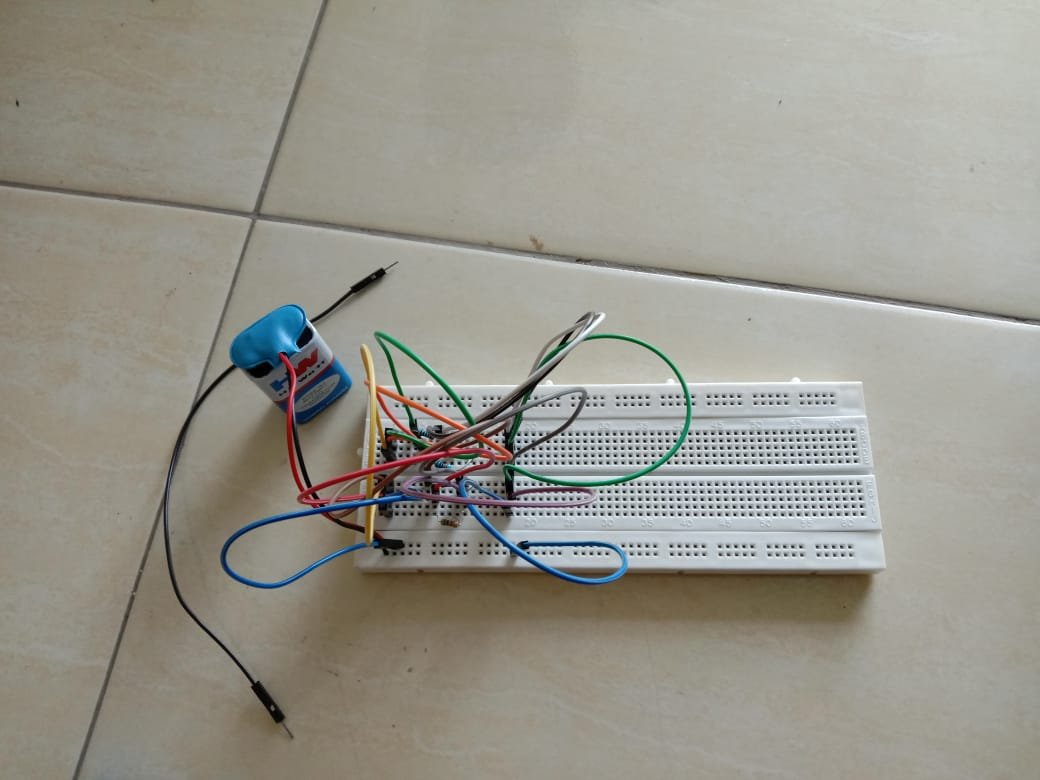
\includegraphics[width=4cm, height=5.5cm]{g1.png}
\end{center}
\end{figure}
\vspace{2cm}

\end{document} %Penulisan Laporan Berakhir
